% =====================================================================================
% Robustness section. Three checks on the correlation result: distribution-free inference,
% grader variance, and threshold transfer.
%
% ALL NUMBERS ARE MEASURED. No placeholders.
%   Source  : results/hpc_vicuna_autodan/ (primary), results/hpc_vicuna_autodan_extthr/
%             (external thresholds), results/hpc_vicuna_autodan/gold_multi.jsonl (5 judgments
%             of every graded response).
%   Scripts : scripts/18_task_a_variance.py, 20_task_b_grader_variance.py,
%             22_task_d_external.py, 23_robustness_figures.py
%   Data    : fusion/taskA/, fusion/taskB/, fusion/taskD/
%
% Place after \S\ref{sec:confound} and before \S\ref{sec:replication}.
% Referenced from \S\ref{sec:corr-measure} (H1), \S\ref{sec:confound}, \S\ref{sec:fusion}
% and \S\ref{sec:limits-corr}, so it must be included wherever those are.
% =====================================================================================

\subsection{Robustness: inference, grader, and calibration}
\label{sec:robustness}

Three properties of the analysis above could in principle be doing the work rather than the
data: the bootstrap's distributional assumptions, the single grader judgment behind every
breach label, and thresholds calibrated on the same benign prompts used to report false
refusals. We tested all three. The composition result survives all of them; two narrower
claims do not, and we say which.

\paragraph{Inference is not doing the work.}
Permuting one member of each pair $10{,}000$ times, which holds both marginals fixed by
construction, makes all fifteen associations significant, and the permutation verdict agrees
with the bootstrap interval on significance for $15/15$ pairs. Cochran's $Q$ across the seven
defenses is $193.4$ ($\mathrm{df}=6$, $p=5\times10^{-39}$), so they are not interchangeable,
and exact-binomial McNemar separates $11$ of the $21$ pairs after Holm correction. The pairs
that do \emph{not} separate are the mid-strength layers among themselves, which is what one
expects if they are close in strength.

One of those non-separations is worth stating because it is easy to conflate with the
correlation result: probe$_{16}$ and probe$_{8}$ do not differ in marginal ASR after
correction ($p=0.039$ uncorrected, $0.309$ after Holm) even though they carry the highest
failure correlation in the study. Indistinguishable marginals and correlated failures are
different claims, and the first does not follow from the second.

\paragraph{The grader is not deterministic, and its variance is not small.}
We judged all $1{,}887$ graded responses five times under an unchanged rubric, model and
temperature. $90.5\%$ of responses are unanimous, $9.5\%$ split, and $4.2\%$ rest on a bare
$3$--$2$ majority. Rebuilding every breach vector from the majority label leaves all fifteen
pairs positive and significant ($q\le1.5\times10^{-3}$), so the correlation result is not an
artefact of one judgment draw.

The individual values move, however, and they move systematically upward: thirteen of fifteen
$\phi$ estimates are larger under majority labels than under the single judgment reported in
Table~\ref{tab:dependency}, by as much as $+0.16$. Resampling one judgment per response gives
a grader-only interval averaging $0.185$ wide against $0.312$ for the behaviour bootstrap ---
about $60\%$ of it. Figure~\ref{fig:forest} shows both. The practical consequence is that
$\Delta$ values within roughly $0.05$ of each other cannot be ordered: among pairs of pairs
separated by less than that, $91\%$ have overlapping grader intervals.

Two marginals also swap rank under majority labels, probe$_{8}$ rising above probe$_{16}$,
which is enough to break the agreement between the row heuristic and the diversity-greedy
search reported in \S\ref{sec:fusion}.

% -------------------------------------------------------------------------------------
\begin{figure}[t]
\centering
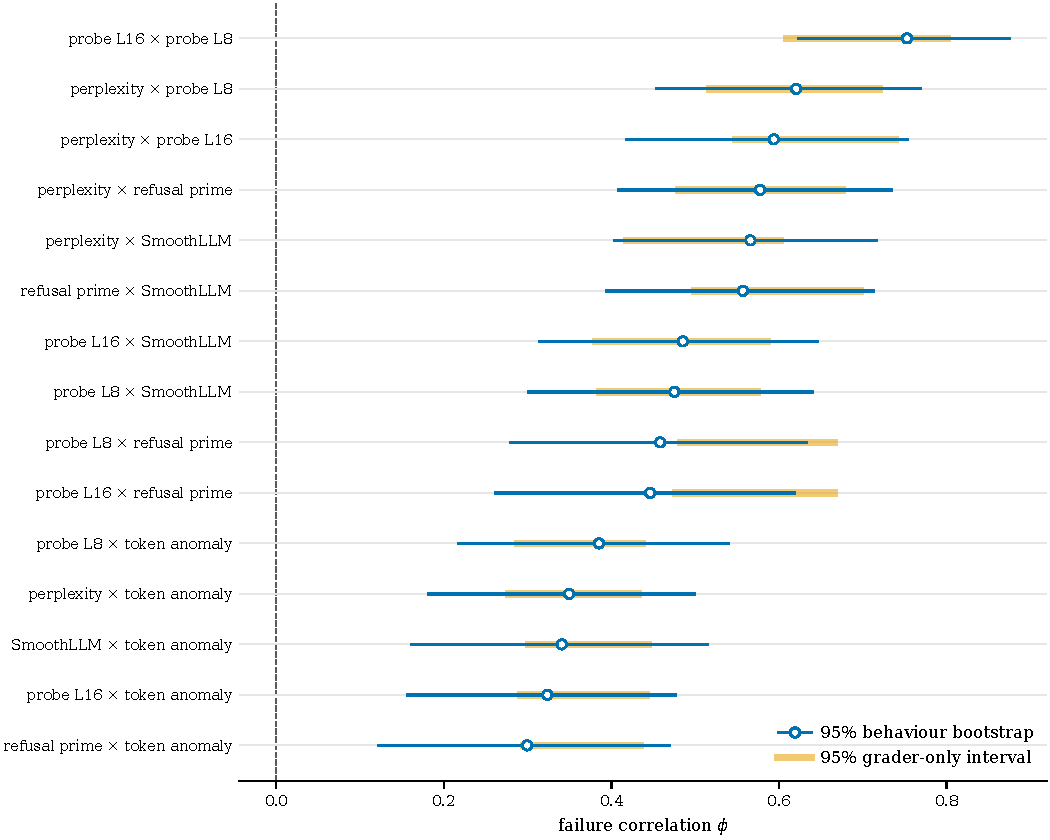
\includegraphics[width=\linewidth]{figures/fig3b_forest_phi.pdf}
\caption{Failure correlation for the fifteen measurable pairs, with two sources of
uncertainty shown separately. The thin interval is the $10{,}000$-resample bootstrap over
behaviours reported throughout this section; the thick band behind it is the grader-only
interval obtained by resampling one of five independent judgments per response. The grader
band averages $60\%$ of the bootstrap's width, so intervals that omit it understate the
uncertainty on every pair.}
\label{fig:forest}
\end{figure}

\paragraph{Threshold transfer.}
Every threshold in the primary run is set on the same $100$ benign prompts later used to
report false-refusal rates, where a $1\%$ target is a single prompt. We re-ran the entire
primary configuration with thresholds set instead on $805$ external instructions, disjoint
from both the evaluation set and the probe's training pool.

\begin{center}
\begin{tabular}{lcccc}
\toprule
Defense & thr.\ in-sample & thr.\ external & FRR in $\to$ ext & ASR in $\to$ ext \\
\midrule
perplexity     & $4.849$   & $6.516$  & $0.08 \to 0.08$ & $0.66 \to 0.67$ \\
token-anomaly  & $0.273$   & $0.523$  & $0.09 \to 0.08$ & $\mathbf{0.35 \to 0.64}$ \\
probe$_{16}$   & $28.924$  & $-5.210$ & $\mathbf{0.08 \to 0.26}$ & $0.68 \to 0.70$ \\
probe$_{8}$    & $110.768$ & $100.593$& $0.09 \to 0.15$ & $0.60 \to 0.66$ \\
\bottomrule
\end{tabular}
\end{center}

Two things follow. The probe's $1\%$ operating point does not transfer: calibrated out of
sample it refuses $26\%$ of the held-out benign set, because the evaluation benign prompts are
matched counterparts to the harmful behaviours and sit far closer to the probe's decision
boundary than ordinary instructions do. And the token-anomaly filter's in-sample threshold was
carrying most of its measured effectiveness, not merely flattering its refusal rate: relaxed to
an out-of-sample operating point its residual ASR nearly doubles.

All fifteen pairs remain positive and significant under external thresholds
($q\le5\times10^{-4}$), several more strongly than in-sample. Figure~\ref{fig:regimes} shows
$\phi$ for every pair under all three regimes; the minimum across the whole grid is $0.300$.

% -------------------------------------------------------------------------------------
\begin{figure}[t]
\centering
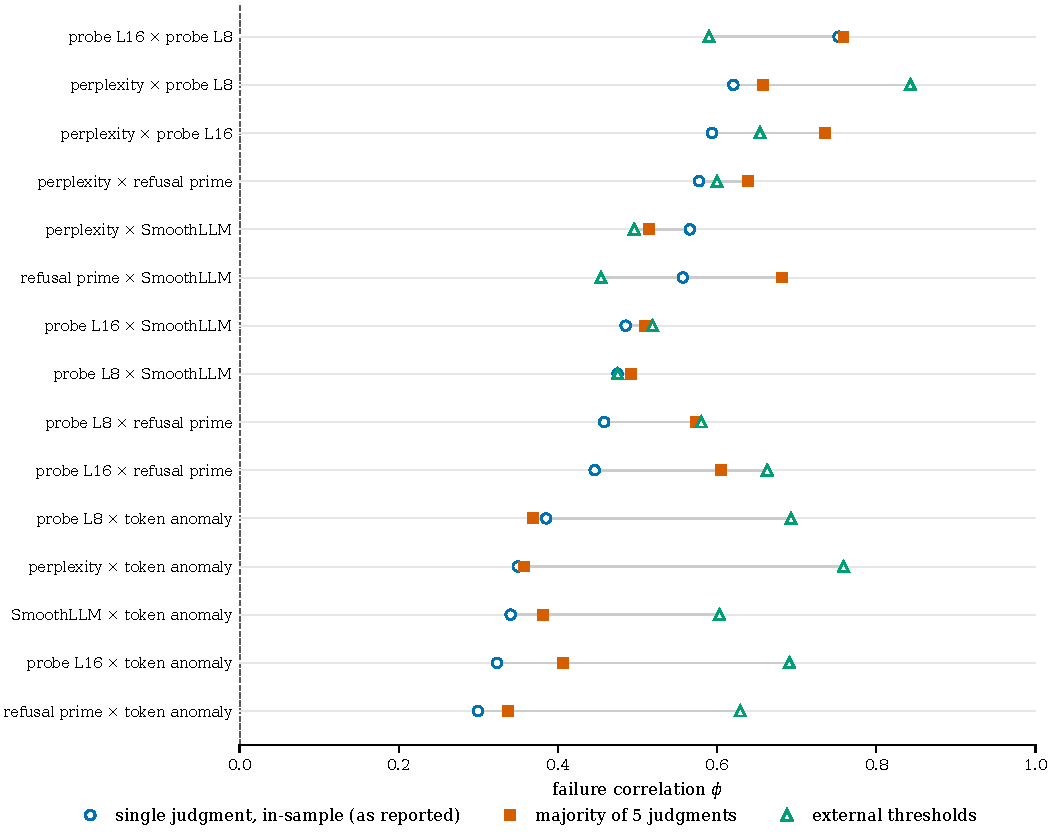
\includegraphics[width=\linewidth]{figures/fig5_regimes_phi.pdf}
\caption{Failure correlation for every measurable pair under the three regimes: the single
judgment and in-sample thresholds reported in Table~\ref{tab:dependency}, majority of five
grader judgments, and thresholds calibrated on an external corpus. Every pair is positive in
every regime --- the minimum over the whole grid is $0.300$ --- while individual values move
by up to $0.4$, which is why we report the direction of these associations rather than their
precise magnitudes.}
\label{fig:regimes}
\end{figure}

\paragraph{What does not survive.}
The mechanism-specific reading of H1 does not, and we retire it rather than report the regime
that favours it. Under majority labels the probe pair still clears the stratified test but its
common odds ratio falls from $159$ to $11.8$, and two \emph{cross-row} pairs begin clearing it
as well. Under external thresholds the pair's stratified test becomes undefined: every
difficulty stratum is saturated --- in the easy strata neither probe is breached, in the hard
strata both are --- so the common odds ratio has an empty concordant cell in every stratum and
is identically zero rather than small. It is the same degeneracy that makes the
semantic-classification row untestable (\S\ref{sec:complementary}), and among the fifteen pairs
it strikes only this one. The single pair that does clear the stratified test under external
thresholds is perplexity~$\times$~probe$_{8}$, which is cross-row.

So the taxonomy of Table~\ref{tab:dependency} remains a useful organising device for choosing
which defenses to combine, and the composition result holds under every perturbation we
applied, but we do not claim that row membership predicts mechanism-specific correlated
failure. On this data that question cannot be settled.
